\begin{wrapfigure}[7]{l}{4.95cm}
  \centering
  \vspace{-0.55cm}
  
\includegraphics[width=0.275\textwidth]{Figures/Problems/Fig 2.1.png}
\end{wrapfigure}
\noindent Mô tả từ trường và các tương tác từ là một bài toán phức tạp hơn so với mô tả các tương tác điện tĩnh. Điều này phần lớn liên quan đến việc không tồn tại các từ tích điểm, do đó nguồn điểm đơn giản nhất của từ trường là lưỡng cực từ. Tuy nhiên, trong nhiều bài toán, ta có thể đưa vào các từ tích điểm nhưng vẫn phải lưu ý rằng các nguồn thực sự của từ trường đều có tổng từ tích bằng 0. Cách tiếp cận này được sử dụng trong bài này để tính toán các từ trường do các nam châm vĩnh cửu tạo ra cũng như đặc điểm của sự tương tác giữa chúng.\\
\indent Theo quan điểm hiện đại, từ trường của nam châm vĩnh cửu được tạo ra bởi các dòng điện từ hóa chạy dọc theo bề mặt của vật bị từ hóa (ý tưởng này ban đầu được A.M. Ampere đưa ra và thường được gọi là giả thuyết Ampere).\\
\begin{figure}[H]
  \centering
  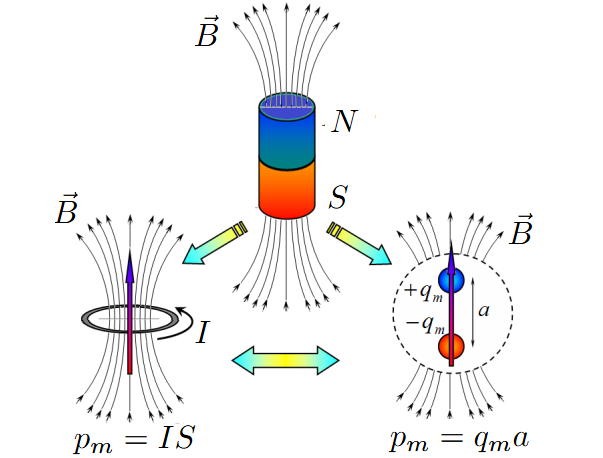
\includegraphics[width=0.55\textwidth]{Figures/Problems/Fig 2.2.png}
\end{figure}
\vspace{-0.4cm}
\noindent Theo đó, một nam châm hình trụ nhỏ có thể được xem như một vòng dây có dòng điện chạy qua. Đại lượng đặc trưng cho vòng dây này là moment từ, được xác định bởi:
\begin{equation*}
  p_m = IS
\end{equation*}
với $I$ là cường độ dòng điện trong vòng dây và $S$ là diện tích hình phẳng giới hạn bởi vòng dây.\\
\indent Một cách tiếp cận thay thế để mô tả từ trường của nam châm là xem xét trường của lưỡng cực từ - một hệ gồm hai từ tích điểm ($+q_m$ và $-q_m$) nằm cách nhau một khoảng $a$ rất nhỏ. Moment từ trong trường hợp này có dạng:
\begin{equation*}
  p_m = q_m a
\end{equation*}
Lưu ý rằng cả hai cách mô tả từ trường chỉ đúng với các điểm cách xa nguồn (nam châm, vòng dây hoặc lưỡng cực từ) nhiều lần so với kích thước của nguồn. Giả sử điều kiện này được thoả mãn trong bài toán hiện tại.\\
\vspace{-0.5cm}
\begin{wrapfigure}[7]{r}{4.5cm}
  \centering
  \vspace{-0.55cm}
  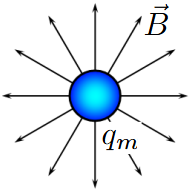
\includegraphics[width=0.2\textwidth]{Figures/Problems/Fig 2.3.png}
\end{wrapfigure}
\indent Từ tích điểm $q_m$ tạo ra một từ trường có vector cảm ứng từ được xác định bởi:
\begin{equation*}
  B = \frac{\mu_0 q_m}{4\pi R^2}
\end{equation*}
trong đó $R$ là khoảng cách từ từ tích điểm đến điểm quan sát trường, và $\mu_0 = 4\pi \times 10^{-7}~\text{Tm/A}$ là độ từ thẩm trong chân không. Bên cạnh đó, lực từ tác dụng lên một đơn cực $q_m$ nằm trong từ trường $\vec{B}$ có dạng:
\begin{equation*}
  \vec{F} = q_m \vec{B}
\end{equation*}
\indent Từ tính của một nam châm vĩnh cửu được đặc trưng bởi độ từ hóa dư $M_R$, được xác định bởi số moment từ trên một đơn vị thể tích:
\begin{equation*}
  M_R = \frac{p_m}{\Delta V}
\end{equation*}
Giá trị này thường được ghi trong thông số kỹ thuật của nam châm. Bên cạnh độ từ hóa dư, người ta còn sử dụng đại lượng:
\begin{equation*}
  B_R = \mu_0 M_R
\end{equation*}
được gọi là cảm ứng từ dư (tức là cảm ứng từ trong lòng nam châm).\\
\indent Lưu ý rằng, hiện tại ta vẫn chưa phát hiện các từ tích, vì vậy các đại lượng $q_m$ không nên xuất hiện trong kết quả cuối cùng. Các kết quả phải được biểu diễn thông qua các đặc trưng thực tế của nam châm – moment từ $p_m$ và độ từ hóa $M_R$.

\subsection*{Phần 1: Đặc trưng của nam châm}
\begin{wrapfigure}[7]{r}{5cm}
  \centering
  \vspace{-0.55cm}
  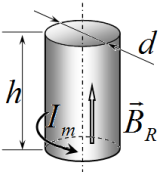
\includegraphics[width=0.2\textwidth]{Figures/Problems/Fig 2.4.png}
\end{wrapfigure}

\noindent Trong bài toán này, xét một nam châm hình trụ làm từ vật liệu Neodymium với các đặc điểm sau:
\begin{itemize}
  \item Đường kính nam châm: $d = 4{,}0~\text{mm}$;
  \item Chiều cao nam châm: $h = 10{,}0~\text{mm}$;
  \item Cảm ứng từ dư: $B_R = 1{,}4~\text{T}$ và hướng dọc theo trục chính nam châm;
  \item Khối lượng riêng của vật liệu: $\rho_{\text{Nd}} = 7{,}6 \times 10^3~\text{kg/m}^3$.
\end{itemize}
Thực hiện các yêu cầu sau:
\begin{enumerate}
  \item Tính khối lượng $m$ của nam châm.
  \item Tính moment từ $p_m$ của nam châm.
  \item Xác định dòng điện từ hóa $I_m$ chạy dọc theo mặt bên của nam châm.
\end{enumerate}

\subsection*{Phần 2: Từ trường của nam châm}
\noindent Xét từ trường do từ tích điểm $q_m$ tạo ra. Từ tích này nằm tại gốc tọa độ trên trục $z$. Vị trí của một điểm bất kỳ được xác định bằng toạ độ $z$ và khoảng cách $r$ tới trục $z$. Trong trường hợp này, cảm ứng từ $\vec{B}^{(0)}$ có thể được phân tích thành hai thành phần: thành phần hướng dọc theo trục $z$: $\vec{B}^{(0)}_z(r,z)$ và thành phần xuyên tâm: $\vec{B}^{(0)}_r(r,z)$.
\begin{figure}[H]
  \centering
  \begin{subfigure}[b]{0.49\textwidth}
    \centering
    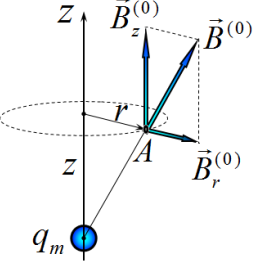
\includegraphics[width=0.5\textwidth]{Figures/Problems/Fig 2.5.png}
  \end{subfigure}
  \hfill
  \begin{subfigure}[b]{0.49\textwidth}
    \centering
    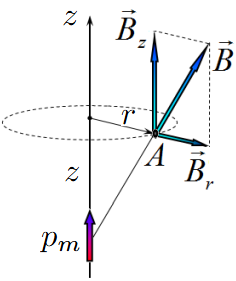
\includegraphics[width=0.5\textwidth]{Figures/Problems/Fig 2.6.png}
  \end{subfigure}
\end{figure}

\begin{enumerate}
  \item Thiết lập biểu thức cho $B^{(0)}_z(r,z)$ và $B^{(0)}_r(r,z)$ theo $r$ và $z$.
\end{enumerate}
\noindent Bây giờ bạn cần khảo sát từ trường do nam châm hình trụ đã mô tả ở trên tạo ra. Để tính toán trường này, ta có thể coi nó trùng với từ trường của một lưỡng cực từ.
\begin{enumerate}
  \setcounter{enumi}{1}
  \item Phác hoạ từ phổ của từ trường do lưỡng cực từ (nam châm hình trụ) tạo ra.
\end{enumerate}
\noindent Giả sử tại gốc của trục $z$ có một lưỡng cực từ với moment từ $p_m$, hướng dọc theo trục $z$. Vị trí của điểm $A$ bất kỳ được xác định bởi toạ độ $(r,z)$.
\begin{enumerate}
  \setcounter{enumi}{2}
  \item Xác định thành phần trục $B_z(r, z)$ của cảm ứng từ do lưỡng cực từ tạo ra theo $r$ và $z$.
  \item Vẽ đồ thị biểu diễn sự phụ thuộc của thành phần trục $B_z(r, z_0)$ theo $r$ tại giá trị cố định $z_0 > 0$.
  \item Xác định cảm ứng từ $B_z(z)$ trên trục $z$ theo toạ độ $z$.
  \item Xác định thành phần xuyên tâm $B_r(r, z)$ của cảm ứng từ do lưỡng cực từ tạo ra theo $r$ và $z$.
  \item Vẽ đồ thị biểu diễn sự phụ thuộc của thành phần xuyên tâm $B_r(r_0, z)$ theo $z$ tại giá trị cố định $r_0 > 0$.
  \item Tìm toạ độ $z = b$ tại đó độ lớn của $B_z(r_0, z)$ đạt giá trị lớn nhất $B_{\text{max}}$. Tìm giá trị cực đại này.
\end{enumerate}
\underline{{Gợi ý toán học:}}
\begin{equation*}
  F(z + a) \approx F(z) + F'(z) \cdot a \quad \text{với } a \ll z
\end{equation*}
\begin{equation*}
  (1 + x)^\gamma \approx 1 + \gamma x \quad \text{với } x \ll 1
\end{equation*}

\subsection*{Phần 3. Hút và đẩy}
\begin{wrapfigure}[7]{r}{6cm}
  \centering
  \vspace{-0.55cm}\hspace{-1cm}
  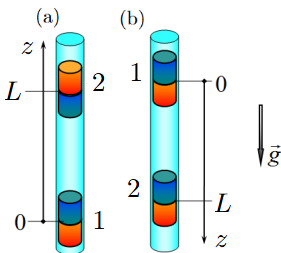
\includegraphics[width=0.28\textwidth]{Figures/Problems/Fig 2.8.png}
\end{wrapfigure}

\noindent Hai nam châm hình trụ giống nhau được đặt trong một ống thuỷ tinh đứng. Nam châm 1 được cố định, nam châm 2 có thể di chuyển tự do dọc theo ống. Khoảng cách giữa các nam châm được rất lớn so với kích thước của chúng. Gia tốc rơi tự do là $g = 9{,}8~\text{m/s}^2$. Trong các ý sau, hãy biểu diễn kết quả theo moment từ $p_m$ và khối lượng $m$ của nam châm.
\begin{enumerate}
  \item Xác định lực tương tác từ giữa hai nam châm theo khoảng cách $z$ giữa chúng.
\end{enumerate}

\begin{enumerate}
  \setcounter{enumi}{1}
  \item Tìm khoảng cách $L$ tại đó nam châm 2 cân bằng. Xét hai trường hợp (a) và (b) theo hướng từ hóa như trên hình.
  \item Chi ra trường hợp nào trong hai trường hợp (a) và (b) có thể được chứng minh bằng thực nghiệm.
  \item Tính toán giá trị số của khoảng cách cân bằng $L$, dựa trên các thông số của nam châm từ Phần 1.
\end{enumerate}

\subsection*{Phần 4. Độ nhớt từ - Dòng Foucault}
\noindent Một nam châm hình trụ được thả vào một ống nhôm mỏng dài nằm thẳng đứng. Bán kính trong của ống là $r_0 = 3{,}0~\text{mm}$, độ dày thành ống là $h_0 = 0{,}30~\text{mm}$. Điện trở suất của nhôm là $\rho = 2{,}8 \times 10^{-8}~\Omega \cdot \text{m}$. Khối lượng và moment từ của nam châm là $m$ và $p_m$ đã biết.\\
\indent Giả sử nam châm rơi với vận tốc không đổi $V$. Xét một vòng tròn mỏng có độ dày $\Delta z$ tại khoảng cách $z$ từ tâm nam châm. Tại các mục 4.1 – 4.4, hãy biểu diễn kết quả thông qua các tham số $b$ và $B_{\text{max}}$ đã tìm được trong ý 2.8.
\begin{figure}[H]
  \centering
  \vspace{0.5cm}
  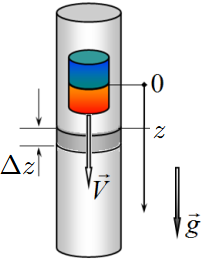
\includegraphics[width=0.2\textwidth]{Figures/Problems/Fig 2.9.png}
\end{figure}

\begin{enumerate}
  \item Xác định cường độ dòng điện cảm ứng $\Delta I$ chạy qua vòng $\Delta z$.
  \item Xác định công suất nhiệt sinh ra trong ống khi nam châm chuyển động.
  \item Xác định lực ma sát từ do dòng Foucault tác dụng lên nam châm đang chuyển động.
  \item Xác định vận tốc rơi ổn định $V$ của nam châm trong ống.
  \item Tính toán giá trị số của vận tốc rơi, dựa trên các thông số của nam châm đã được giới thiệu trong Phần 1.
\end{enumerate}
\underline{Chú thích:} Sự phụ thuộc của thành phần xuyên tâm của từ trường tại thành ống có thể được xấp xỉ bằng hàm bậc thang như hình vẽ. Sử dụng các tham số $b$ và $B_{\text{max}}$ từ mục 2.8. Nếu bạn chưa tìm được các đáp án từ 2.8, trong phần này có thể xem như chúng đã biết.\\
\begin{figure}[H]
  \centering
  \vspace{-0.5cm}
  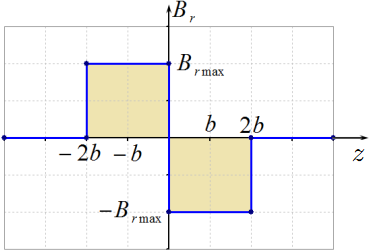
\includegraphics[width=0.4\textwidth]{Figures/Problems/Fig 2.10.png}
\end{figure}